\documentclass[a4paper,12pt]{article}
\usepackage[slovene]{babel}
\usepackage[utf8]{inputenc}
\usepackage[T1]{fontenc}
\usepackage{lmodern}
\usepackage{amsmath,amsfonts}
\usepackage{enumitem}
\usepackage{graphicx}
\usepackage{subfigure}
\usepackage{mathtools}
\pagenumbering{roman}

\begin{document}

\newcommand{\N}{\mathbb{N}}
\newcommand{\R}{\mathbb{R}}
\newcommand\sbullet[1][.5]{\mathbin{\vcenter{\hbox{\scalebox{#1}{$\bullet$}}}}}
%\theoremstyle{definition} % tekst napisan pokoncno
\newtheorem{definicija}{Definicija}[section]
\newtheorem{primer}[definicija]{Primer}
\newtheorem{opomba}[definicija]{Opomba}


\title{Diskretne Coonsove ploskve}
\author{Matej Rojec, Vito Rozman}
\date{\today}

\maketitle


\newpage

\tableofcontents
\listoffigures

\newpage

\section{Uvod}

V seminarski nalogi bomo obravnavali površine, ki interpolirajo dane mejne krivulje. 
Te površine imenujemo diskretne Consove ploskve, ki jih dobimo z reševanjem linearnega sistema.


Eden od najstarejših problemov v Računalniško podprtem geometrijskem oblikovanju je problem, 
kjer imamo podane štiri robne krivulje, radi pa bi poiskali ploskev z danimi robnimi krivuljami. 
Torej podane imamo robne krivulje $$x(u,0), x(u,1), x(0,v),  x(1,u)$$, kjer lahko brez škode za 
splošnost predpostavimo da je domena ploskve $x(u,v)$ enotni kvadrat $0 <= u,v <=1$. Znana rešitev 
tega problema je bilinearna mešana Coonsova ploskev, ki je interpolirana z robnimi 
krivuljami, kot: 
\begin{align*}
   \label{continiusCons}
   \mathbf{x}(u,v) =& (1-u)\mathbf{x}(0,v) +u\mathbf{x}(1,v)\\
    & + (1-v)\mathbf{x}(u,0) +v\mathbf{x}(u,v) \\
   & - 
   \begin{bmatrix} 
      1-u & u 
   \end{bmatrix}
   \begin{bmatrix} 
      \mathbf{x}(0,0)& \mathbf{x}(0,1)\\
      \mathbf{x}(1,0)&\mathbf{x}(1,1) 
   \end{bmatrix}
   \begin{bmatrix}
      1-v\\
      v
   \end{bmatrix}
\end{align*}


\section{Diskretne Coonsove ploskve}
V bolj modernih uporabah CAD, so mejne krivulje Bezierjeve polinomske krivulje, 
ki jih napenjajo kontrolni poligoni. 
\begin{definicija}
    Naj bodo dane točke $\mathbf{b}_0, \mathbf{b}_1, \dots, \mathbf{b}_n$. Potem je Bezierjeva 
    krivulja podana s polinomsko paramerizacijo $\mathbf{p}: [0,1] -> \R^d$ s predpisom 
    $$\mathbf{p}(t) = \sum_{i=0}^n \mathbf{b}_{i} B_i^n(t),$$
    kjer je $B_i^n(t) = \binom{n}{i} t^i (1-t)^{n-i}$, za $i = 0, 1,\dots,n$. Točkam $\mathbf{b}_i$
    pravimo kontolne točke.
\end{definicija}

\begin{definicija}
    Bézierjevo ploskev $\mathbf{p} : [0,1]^2 \rightarrow \R^3$ iz tenzorskega produkta stopnje 
    $(m, n) \in \N \times \N$ definiramo s parametrizacijo:
    $$\mathbf{p}(u,v) := \sum_{i=0}^m \sum_{j=0}^n \mathbf{b}_{i,j} B_i^m(u)B_j^n(v),$$
    kjer sta $(u,v) \in [0,1]^2$ ter $(\frac{i}{m}, \frac{j}{n})$
    domenske točke, ki ustrezajo kontrolni točki $\mathbf{b}_{i,j}$.
\end{definicija}


V tem primeru imamo podane kontrolne točke $b_{i,j}$ opremljene z 
parametroma $(u,v)$ predstavljen s shemo: 
$$
\begin{matrix}
   \mathbf{b}_{0,0}  &\mathbf{b}_{1,0} & \ldots &\mathbf{b}_{m-1,0} &\mathbf{b}_{m,0} \\
   \mathbf{b}_{0,1}  &                 &        &                   &\mathbf{b}_{m,1} \\
   \vdots            &                 &        &                   &  \vdots\\
   \mathbf{b}_{0,n-1} &                &        &                    &\mathbf{b}_{m,n-1} \\ 
   \mathbf{b}_{0,n}  &\mathbf{b}_{1,n} & \ldots &\mathbf{b}_{m-1,n} &\mathbf{b}_{m,n} 
\end{matrix}
$$

   

Sedaj lahko primer diskritiziramo in robne krivulje zapišemo s štirimi 
Bezierjevimi krivuljami:
\begin{align*}
    &\mathbf{p}(u,0) =\sum_{i=0}^m \mathbf{b}_{i,0} B_i^n(u), \qquad
    \mathbf{p}(u,1) =\sum_{i=0}^m \mathbf{b}_{i,n} B_i^n(u),  \\
    &\mathbf{p}(0,v) =\sum_{j=0}^n \mathbf{b}_{0,j} B_j^n(v), \qquad
    \mathbf{p}(1,v) =\sum_{j=0}^n \mathbf{b}_{m,j} B_j^n(v),  \\
 \end{align*}
Tako se notranje toče izražajo z formulo: 
\begin{align*}
   \mathbf{b}_{i,j} =& (1 - \frac{i}{m})\mathbf{b}_{0,j} +\frac{i}{m}\mathbf{b}_{m,j}\\
    & + (1 - \frac{j}{n})\mathbf{b}_{i,0} +\frac{j}{n}\mathbf{b}_{i,n}\ \\
   & - 
   \begin{bmatrix} 
      1 - \frac{i}{m} & \frac{i}{m}
   \end{bmatrix}
   \begin{bmatrix} 
      \mathbf{b}_{0,0} & \mathbf{b}_{0,1}\\
      \mathbf{b}_{1,0} & \mathbf{b}_{1,1}
   \end{bmatrix}
   \begin{bmatrix}
      1 - \frac{j}{n}\\
      \frac{j}{n}
   \end{bmatrix}
\end{align*}
za $i = 1,2,\dots,m-1$ in $j = 1,2,\dots,n-1$. Izkaže se, da je kontrolni poligon ploskev, 
ki jo omejujejo robne krivulje,   enak kontrolnemu poligonu, ki ga dobimo z opisano metodo. 
»Morda zanimivo: za določene oblike rabimo definirati samo robne krivulje«.

\begin{figure}[ht!]
   \centering
   \subfigure[Primer robnih točk]{
   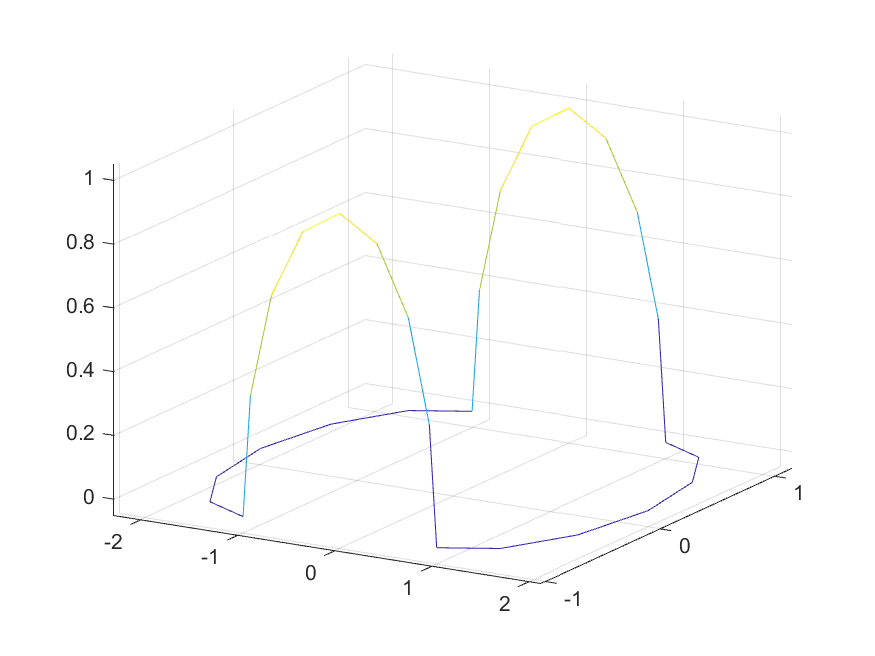
\includegraphics[width=0.45\textwidth]{ogrodje.png}
   }
   \subfigure[Primer ogrodja]{
   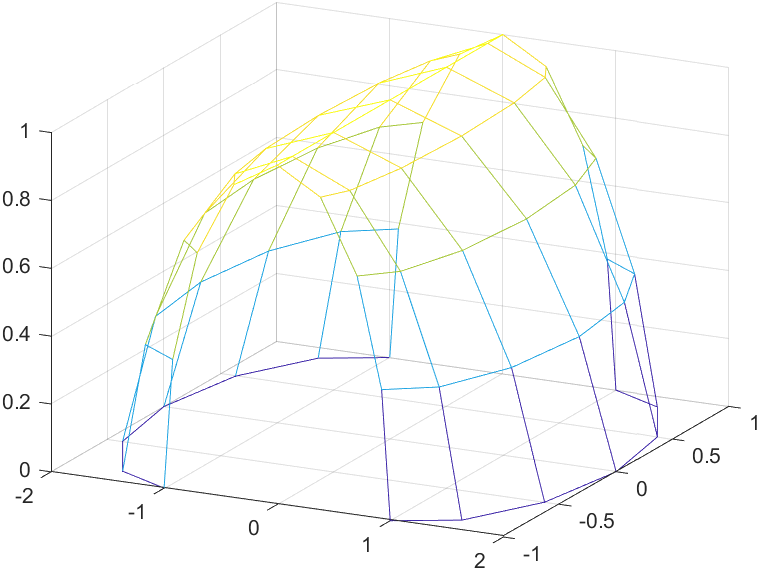
\includegraphics[width=0.45\textwidth]{dodatne_kont_t.png}
   }
   
   \subfigure[Coonsova ploskv na ogrodju]{
   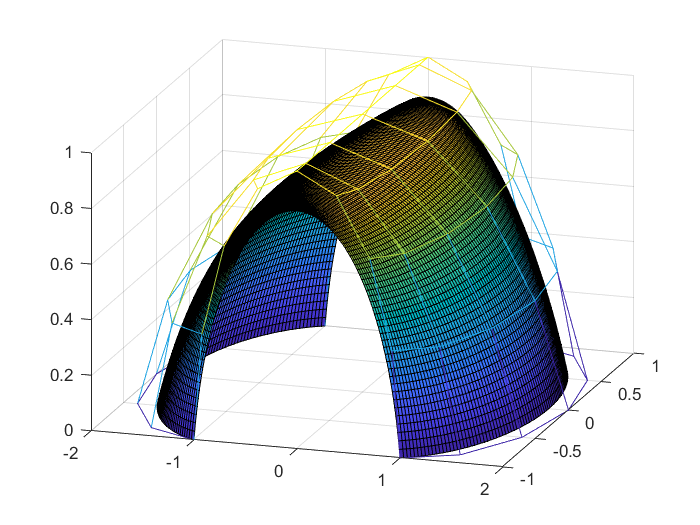
\includegraphics[width=0.5\textwidth]{primer_krivulje.png}
   }   
   \caption{Primer konstrukcije Coonsove ploskve}
\label{fig:whatever}
\end{figure}


\newpage




\section{Lastnosti Coonsovih ploskev}

%\subsection{Minimziraje zasuka}
%Coonsova ploskve minimzirajo zasuk, definiran kot:
%\begin{equation}
%   \label{eq:min}
%   \int_{[0,1]^2} \left( \frac{\partial^2}{\partial u \partial v}\mathbf{p}(u,v) \right)^2 dS.
%\end{equation}
%Torej coonsova ploskev doseže minimum izraza.
%Posledica tega je, da so Coonsova ploskve lahko v primerih preveč ravne in ne interpolirajo dobro kontrolnih točk.
%Taka ploskev prav tako zadošča Euler-Lagrangovi parcialni diferencialni enačbi, torej velja:
%\begin{equation}
%   \label{eq:pde}
%    \frac{\partial^4}{\partial u^2 \partial v^2}\mathbf{p}(u,v) = 0.
%\end{equation}

\subsection{Ohranjanje Coonsove ploskve}

Naj bo Cooncova ploskev definirana nad domeno $D = [0,1]^2$. Lahko izberemo dve 
točki $(u_0,v_0)$ in $(u_1,v_1)$ ki razpenjata pravokotnik $R$ v domeni $D$. 
Štiri mejne krivulje pod-Consove ploskve definiranega na $R$ se preslikajo 
v štiri krivulje na prvotno Consovo ploskev. Izkaže se da pod-Coonsova ploskev 
definirana na $R$ je prvotna Coonsova ploskev zožana na območje $R$. To načelo 
lahko uporabimo na diskretni $3 \times 3$ Consovi ploskivi
$$
\begin{matrix} 
   \mathbf{b}_{i-1,j-1} & \mathbf{b}_{i-1,j} & \mathbf{b}_{i-1,j+1}\\
   \mathbf{b}_{i,j-1} & \mathbf{b}_{i,j} & \mathbf{b}_{i,j+1}\\
   \mathbf{b}_{i+1,j-1} & \mathbf{b}_{i+1,j} & \mathbf{b}_{i+1,j+1}
\end{matrix}
$$ 
Če poznamo robne točke lahko notranjo točko $\mathbf{b}_{i,j}$ določimo na sledeč način: 
\begin{align*}
   \mathbf{b}_{i,j} =& -\frac{1}{4}(\mathbf{b}_{i-1,j-1} + \mathbf{b}_{i+1,j-1} +
      \mathbf{b}_{i-1,j+1} + \mathbf{b}_{i+1,j+1}) \\
      &+\frac{1}{2}(\mathbf{b}_{i-1,j} + \mathbf{b}_{i,j-1}+
      \mathbf{b}_{i,j+1} + \mathbf{b}_{i+1,j}).\\
\end{align*}
kar lahko krajše zapišemo z masko: 
$$
\mathbf{b}_{i,j} = -\frac{1}{4} \times 
\begin{matrix*}[r]
-1 && 2 && -1 \\
2 && \sbullet && 2\\
-1 && 2 && -1
\end{matrix*}
$$
Ker je mreža sestavljena iz $(m+1)\times(n+1)$ kontrolnih točk, dane pa imamo samo robne
točke lahko ostalih $(m-1)\times(n-1)$ enlično določimo z zgornjo masko. Določitev točk se prvede
na sistem $(m+1)\times(n+1)$ linearnih enačb.

Oglejmo si $3 \times 3$ masko s splošnimi parametri, kjer se elemt izraža na sledeč način
$$
\mathbf{b}_{i,j} =  \quad 
\begin{matrix*}[r]
\alpha && \beta && \alpha \\
\beta && \sbullet && \beta \\
\alpha && \beta && \alpha
\end{matrix*}
$$
V primeru da sta $(\alpha, \beta) = (-0.25, 0.5)$ dobimo splošno Consovo
ploskvo. Vedno bomo privzeli, da velja $4\alpha + 4\beta = 1$, saj 
tako ohranjamo afinost maske. S perturbiranjem parametrov 
$\alpha$ in $\beta$ dobimo torej nov razred kontrolnih shem, imenujemo jih stalne 
krivulje (ang. permanence patches). V članku \cite{DCP}  so raziskovali
vpliv $\alpha$ na optimalno oblike ploskve. Ugotovili so, da za izbrana $m$ in $n$
ni vedno ene optimalne vrednosti za $\alpha$, ki bo dala dobro obliko ploskve.

\section{Stalne Coonsove ploskve}


Ena kontrolna točka navadne Consove ploskve je odvisna od osem obrobnih točk, 
torej gre za lokalno odvisnost. V primeru ko govorimo o stalnih ploskvah 
($\alpha \neq  -0.25$), je točka odvisna od vseh mejnih točk, zato govorimo 
o globalni odvisnosti. Ta odvisnost nam potencialno lahko pripomore pri ustvarjanju 
"boljših" krivulj.

Če si ogledamo primer, ko izberemo $\alpha = -0.257$ in rešimo linearni sistem, dobimo "boljšo"
ploskev glede na dane robne rivulje. 
TU BO SLIKA
%\includegraphics*[keyvals]{imagefile}
Dani poligoni izhajajo iz torusnih oblik in z modifikacijo $\alpha$ lahko pridemo do željene oblike.
Kot zanimivost se izkaže da ob izbiri paramatra $\alpha = 0$ in seveda ob upoštevanju afinosti,
dobimo ploskev, katere površina je minimizeranan za dano ogrodje krivulj. To se vidi iz Laplasove parcialne 
diferencialne enačbe
$$\mathbf{x}_{uu} + \mathbf{x}_{vv} = 0.$$


\section{Trikotne stalne Coonsove ploskve}

Mreža trikotne Bezirjeve krivulje je delno linearna površina, zato se v tem primeru porodi vprašanje,
če imam tri robne poligone, ali obstaja "dobra" kontolna mreža ki zapolni omejeno območje. Ideja rešitve je
podobna kot v prejšnem primeru, kjer uporabimo spremenjeno masko oblike:

$$
\mathbf{x} =  \quad 
\begin{matrix*}[r]
          &       &       & \alpha   &       &       & \\
          &       & \beta &          & \beta &       & \\
          & \beta &       & \sbullet &       & \beta & \\
   \alpha &       & \beta &          & \beta &       & \alpha
\end{matrix*}
$$
kjer je zaradi pogoja afinoste ponovno predpostavljeno da $3\alpha + 6\beta = 1$.




















\newpage


\newpage

\begin{thebibliography}{99}
   \bibitem{DCP}
   G.~Farin, F.~Hansford, \emph{Discrete Coons patches}, 
   % popravi Morgan \& Claypool Publishers, 2018.
\end{thebibliography}
\end{document}